Formeln för en triangels area är $\frac{b \cdot h}{2}$.
Utgår man ifrån detta så får man att basen kan representeras av $||\overrightarrow{P_{1}P_{3}}||$ (eller $\overrightarrow{P_{1}P_{2}}$).
Höjden, däremot, går inte att representera direkt utav någon vektorn baserad på punkterna $P_{1}$, $P_{2}$ och $P_{3}$.
För att få höjden tar man $\overrightarrow{P_{1}P_{2}}$ projektion på den linje som har riktningsvektor $\overrightarrow{P_{1}P_{3}}$, 
som blir basen till en triangel med $||\overrightarrow{P_{1}P_{2}}||$ som hypotenusa.
Enligt Pytagoras sats kan man då få höjden på denna nya triangel genom $\sqrt{ ||\overrightarrow{P_{1}P_{2}}||^{2} - (\frac{|\overrightarrow{P_{1}P_{3}}\cdot \overrightarrow{P_{1}P_{2}}|}{||\overrightarrow{P_{1}P_{3}}||})^{2}}$.
Om man sedan multiplicerar denna höjden, med $||\overrightarrow{P_{1}P_{3}}||$ så får man formeln för triangelns area enligt följande:\\
\begin{equation}
        \frac{\sqrt{ ||\overrightarrow{P_{1}P_{2}}||^{2} - (\frac{|\overrightarrow{P_{1}P_{3}}\cdot \overrightarrow{P_{1}P_{2}}|}{||\overrightarrow{P_{1}P_{3}}||})^{2}}\cdot ||\overrightarrow{P_{1}P_{3}}||}{2}
\end{equation}

\begin{center}
    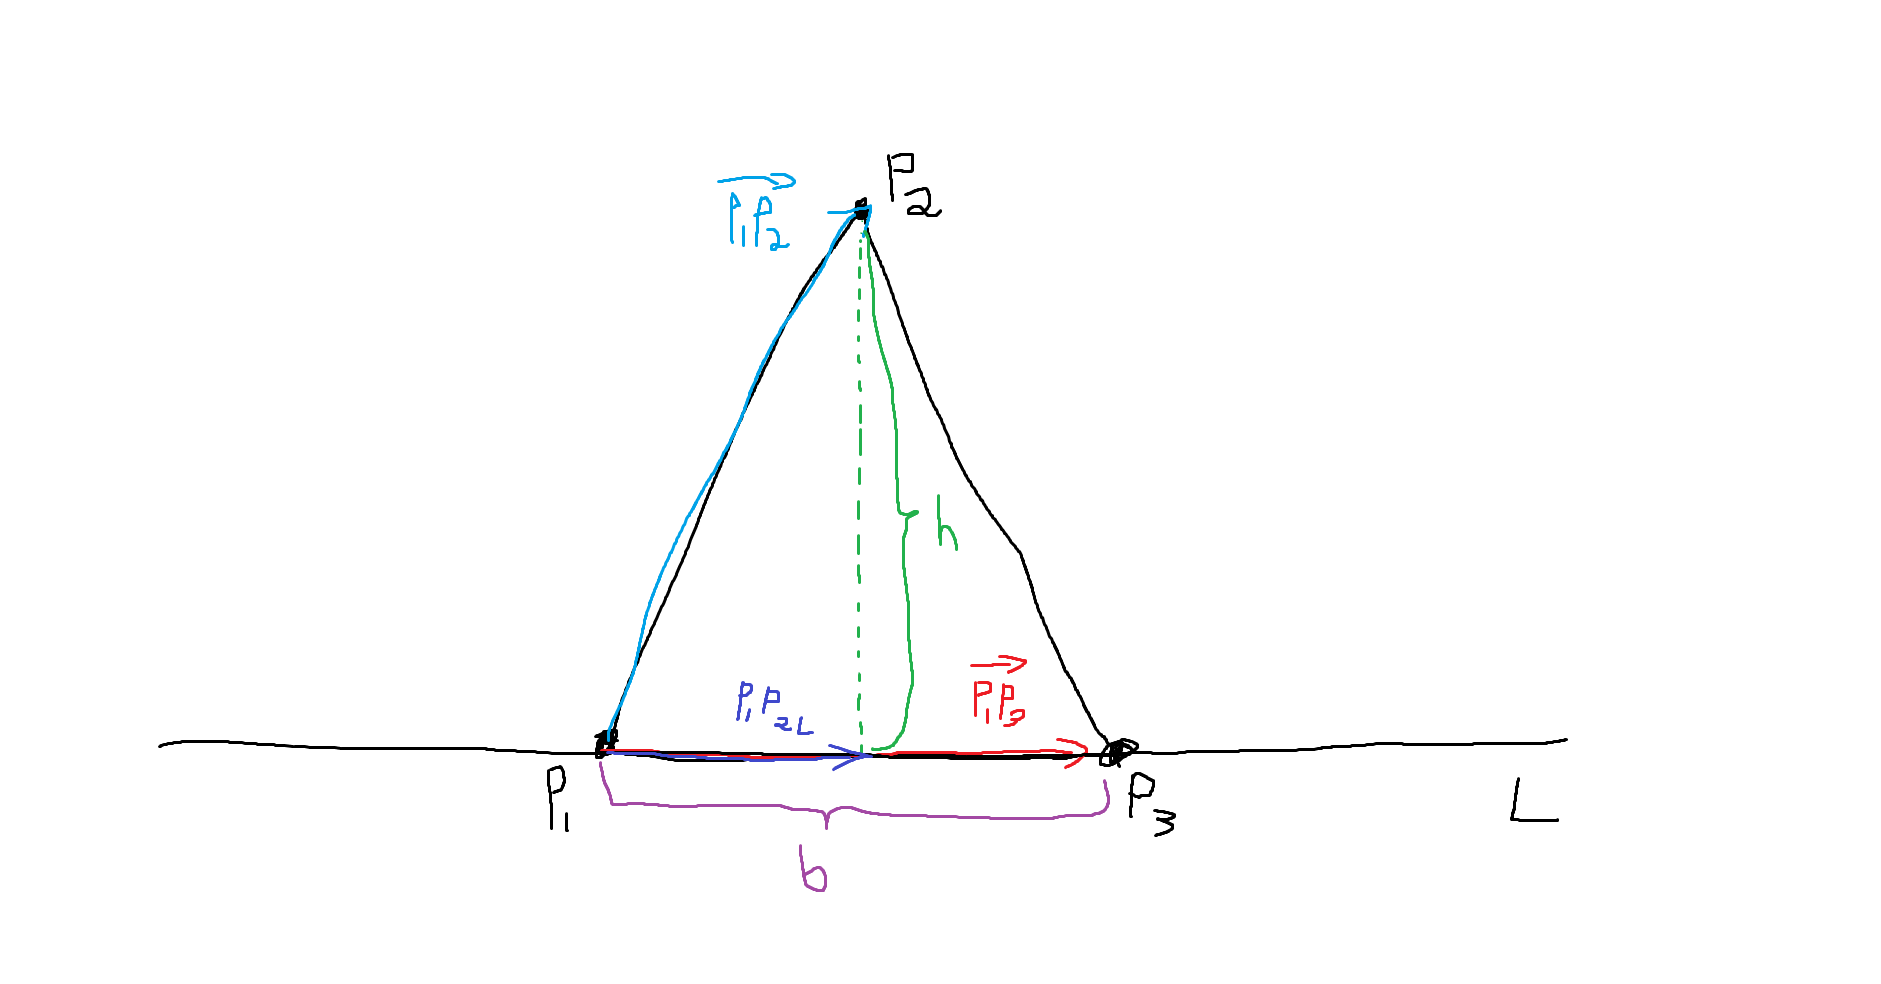
\includegraphics[scale=0.15]{imgs/bild.png}
\end{center}

Om vi sedan applicerar denna formel på triangeln med hörnen $P_{1}=(1,1)$, $P_{2}=(4,2)$ och $P_{3}=(-1,7)$, så har vi vektorerna:\\
\begin{center}
    $\bm{v} = P_{1}-P_{2} = \begin{pmatrix}5\\-5\end{pmatrix}$\\
    $\bm{u}=P_{1}-P_{3} = \begin{pmatrix}2\\-6\end{pmatrix}$\\
\end{center}

Om man sedan kan stoppa in i formeln för att få arean:
\begin{equation}
    \frac{\sqrt{||\bm{v}||^{2}-(\frac{|\bm{u}\cdot \bm{v}|}{||\bm{u}||})^{2}}\cdot ||\bm{u}||}{2}=
    \frac{\sqrt{\sqrt{50}^{2}-(\frac{5\cdot 2 + (-5)\cdot (-6)}{\sqrt{40}})^{2}}\cdot \sqrt{40}}{2}=
    10
\end{equation}